Query 1 requires to forecast average load of each plug and each house in the system. A day is divided into equally spaced slots of different time slices. The time slices are of length 1 min, 5 min, 15 min, 60 min and 120 min. For example, there will be $(24*60/15) = 96$ slots in a day corresponding to the time slice of length 15 min; for the 60 min slice, there will be $(24*60/60) = 24$ slots in a day and so on. The average load forecast is computed over all possible slots of all the time slices.

In order to make a forecast, we use 2 values- current average load and median load for the slot of given time slice. Using these 2 values, we forecast the average load for the next to next slot of the same time slice. We put out a forecast every 30 sec i.e. for each time slice we compute average load whenever we accumulate more data for next 30 seconds.


\subsection{Architecture}
The system consists of a broker process and house processes per house. The broker reads the data file and passes all the events for house id \textit{h} to the corresponding house process as shown in the figure \ref{fig:sysarch1}. House process is responsible for the forecast of average load of house and all the plugs in all households in the house.

\begin{figure}[h]
\begin{center}
\begin{tikzpicture}[scale=0.8, >=stealth', transform shape, shorten >=1pt, node distance=2cm,auto]
\tikzstyle{every state}=[draw=blue!50, very thick, fill=blue!20]
\node[state] (broker) [text width=1.2cm, align=center] {Broker Process};

\node[state] (h2) [right of=broker,text width=1.2cm, align=center, node distance=4cm] {House 2 Process};
\node[state] (h1) [above of=h2,,text width=1.2cm, align=center] {House 1 Process};
\node[state] (h3) [below of=h2,text width=1.2cm, align=center] {House 3 Process};

\path[->] (broker) edge node[midway, sloped, anchor=south] {h1 events} (h1);
\path[->] (broker) edge node[midway] {h2 events} (h2);
\path[->] (broker) edge node[midway, sloped, anchor=south] {h3 events} (h3);
\end{tikzpicture}
\caption{Query 1 System Architecture}
\end{center}
\label{fig:sysarch1}
\end{figure}

In the house process, we keep a 30s accumulator for each plug. Whenever we receive an event for a plug, we increment the accumulator with the load\footnote{For now, we are ignoring events with work values} value in the received event. We store a count of values we receive with the timestamp within last 30s in order to calculate average later on. We also keep load value accumulators for different time slices (1m, 5m, 15m, 60m and 120m). 

As soon as we receive an event crossing the 30s time window, we add the value of the 30s accumulator and the count into the time slice accumulators and counts. We reinitialize the 30s accumulator to the load value in the received event and count to 1. A forecast is made for all the current time slots, whose slot boundary is crossed i.e. the received event does not belong to the current slot. We predict average load for next to next slot for such time slices using the average load and the historical median of the corresponding slot. The accumulators and count for such time slices get reset to 0. We output forecast as 0 if all the data is missing in a slot for a time slice. Note that, the above algorithm is based on the assumption that the timestamp of events coming from the broker never decreases. We, therefore, can make the forecast whenever any event corresponding to any plug in the house, crossing the current time slot for a time slice is received.

We defined a Median Container (MC) to compute exact median in case of query 1. MC provides an interface to insert a new element and retrieve median of all the elements currently in the container. We insert the average load of a plug or house for a given slot of fixed time slice into the container as soon as we compute it. The container returns the exact median of all the average values inserted into it.

\subsection{Median Algorithm (MC)}
We have used an exact algorithm to compute median of average loads in case of Query 1. We store all the previous days average loads in the container for a given time slot of any time slice.

We maintain two heaps inside the container. One of the heap is a min heap and stores half of the higher values inserted into the container. On the other hand, second heap is a max heap and stores the other half of the lower values. If the total number of values inserted, are odd, we keep the median value in a separate variable. Now following cases can occur-
\begin{itemize}
\item If the total number of values are odd, the extra variable stores the median.
\item If the total number of values are even, the median would be average of the root of both the heaps.
\end{itemize}

When a new value is inserted into the container, following cases can occur-
\begin{itemize}
\item If the total number of elements are odd before insertion, first we find out the lower value between the inserted value and the extra element. We, then, insert the lower value to the max heap and the other value to the min heap.
\item If the total number of elements are even before insertion, we insert the value in either min or max heap such that the invariant that the max heap contains the lowest values and the min heap contains the highest values is maintained. We keep one extra element in a separate variable as explained before.
\end{itemize}

\subsection{Prediction Model}

\subsection{Experimental Evaluation}
We executed our solution in a Virtual Machine Cluster. The broker is running on kvm based 2.1GHz virtual machine with 1 GB memory attached to a 10 Gbit local area network running Ubuntu 12.04. The house processes also run on a similarly configured Virtual Machines. We did experiments running house processes on 1,2 and 4 Virtual Machines dividing equal (or 1 more) number of processes to each VM.

For throughput calculations, we redirected the output to the null file. Throughput will simply be the total number of input events divided by the total time taken in processing all the events. We did each experiment three times and took the average of the three throughput values.

\begin{figure}[h]
\begin{center}
	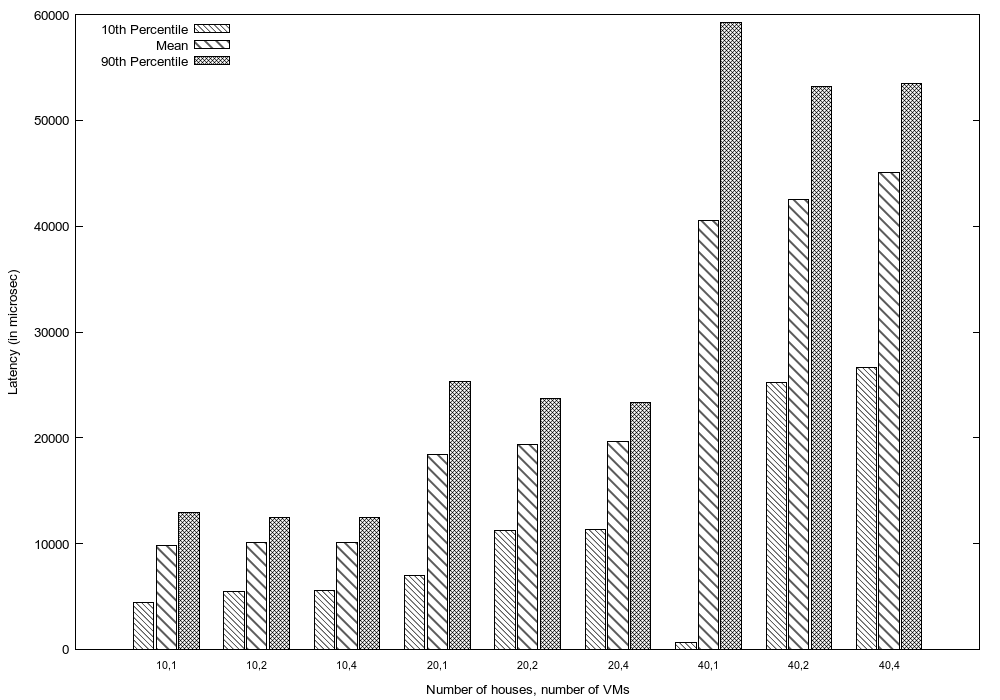
\includegraphics[scale=0.45]{img/q1_latency}
\end{center}
\end{figure}

As we increase the number of virtual machines, the latency values do not change much because the broker becomes the bottleneck. The disk read in the broker becomes limits the scalability of the system. On the other hand, throughput remains nearly constant in all the experiments.

\begin{figure}[h]
\begin{center}
	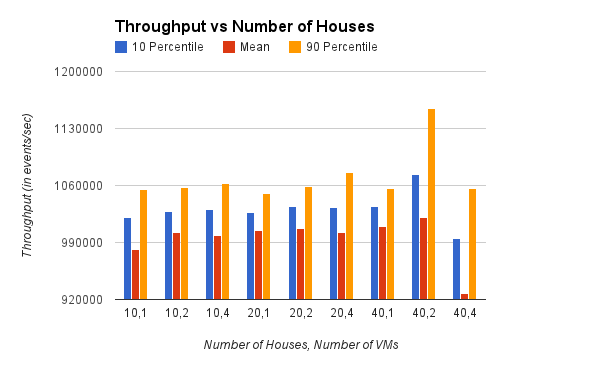
\includegraphics[scale=0.45]{img/q1_throughput}
\end{center}
\end{figure}